\documentclass[11pt]{article}

\usepackage{amsmath}
\usepackage{amssymb}

\usepackage{graphicx}
\usepackage{tikz}

\usepackage{ytableau}


\title{Walks, paths, and degrees, \\ UMTYMP Advanced Topics, Fall 2020}
\date{}


\begin{document}


\maketitle



An \emph{Eulerian walk} in a graph $G$ is a walk that crosses each edge exactly once. An \emph{Eulerian circuit} is an Eulerian walk that's a circuit (a closed walk).

\begin{enumerate}

\item For each of the following graphs: does the graph have an Eulerian walk? Does it have an Eulerian circuit?
\[ (a) 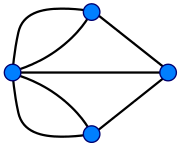
\includegraphics[width=1in]{konigsberg.png} \qquad \qquad (b) 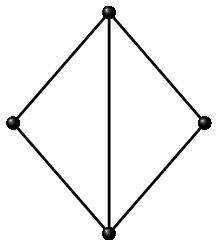
\includegraphics[width=1in]{kite.png} \qquad \qquad (c) 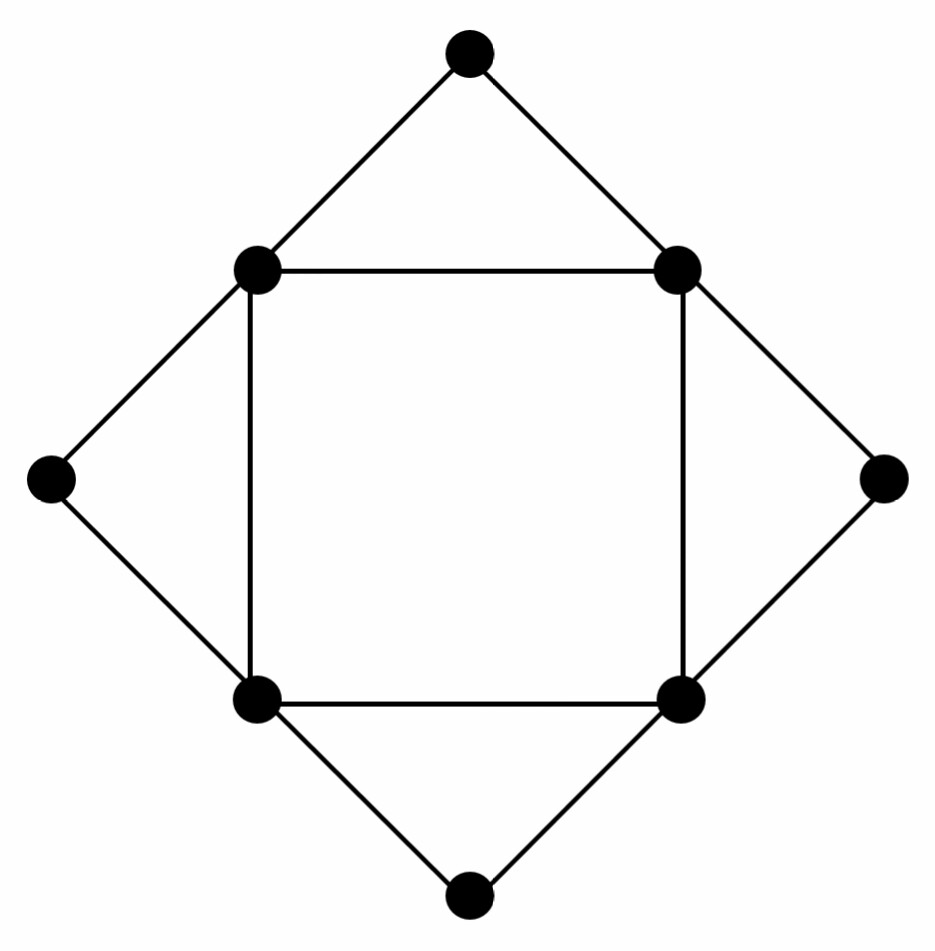
\includegraphics[width=1.2in]{eulerian.png} \]

\end{enumerate}

A \emph{Hamiltonian path} in a graph $G$ is a walk that visits every vertex exactly once. A \emph{Hamiltonian cycle} in a graph $G$ is a circuit that visits every vertex exactly once (except that, being a circuit, it ends at the vertex it starts at).

\begin{enumerate}

\setcounter{enumi}{1}

\item For each of the following graphs: does the graph have a Hamiltonian path? Does it have a Hamiltonian cycle?
\[ (a) 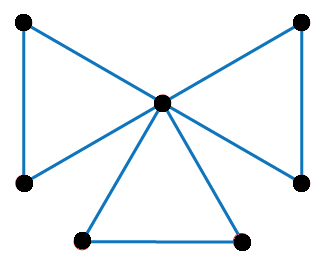
\includegraphics[width=1in]{nonhamilton.png} \qquad \qquad (b) 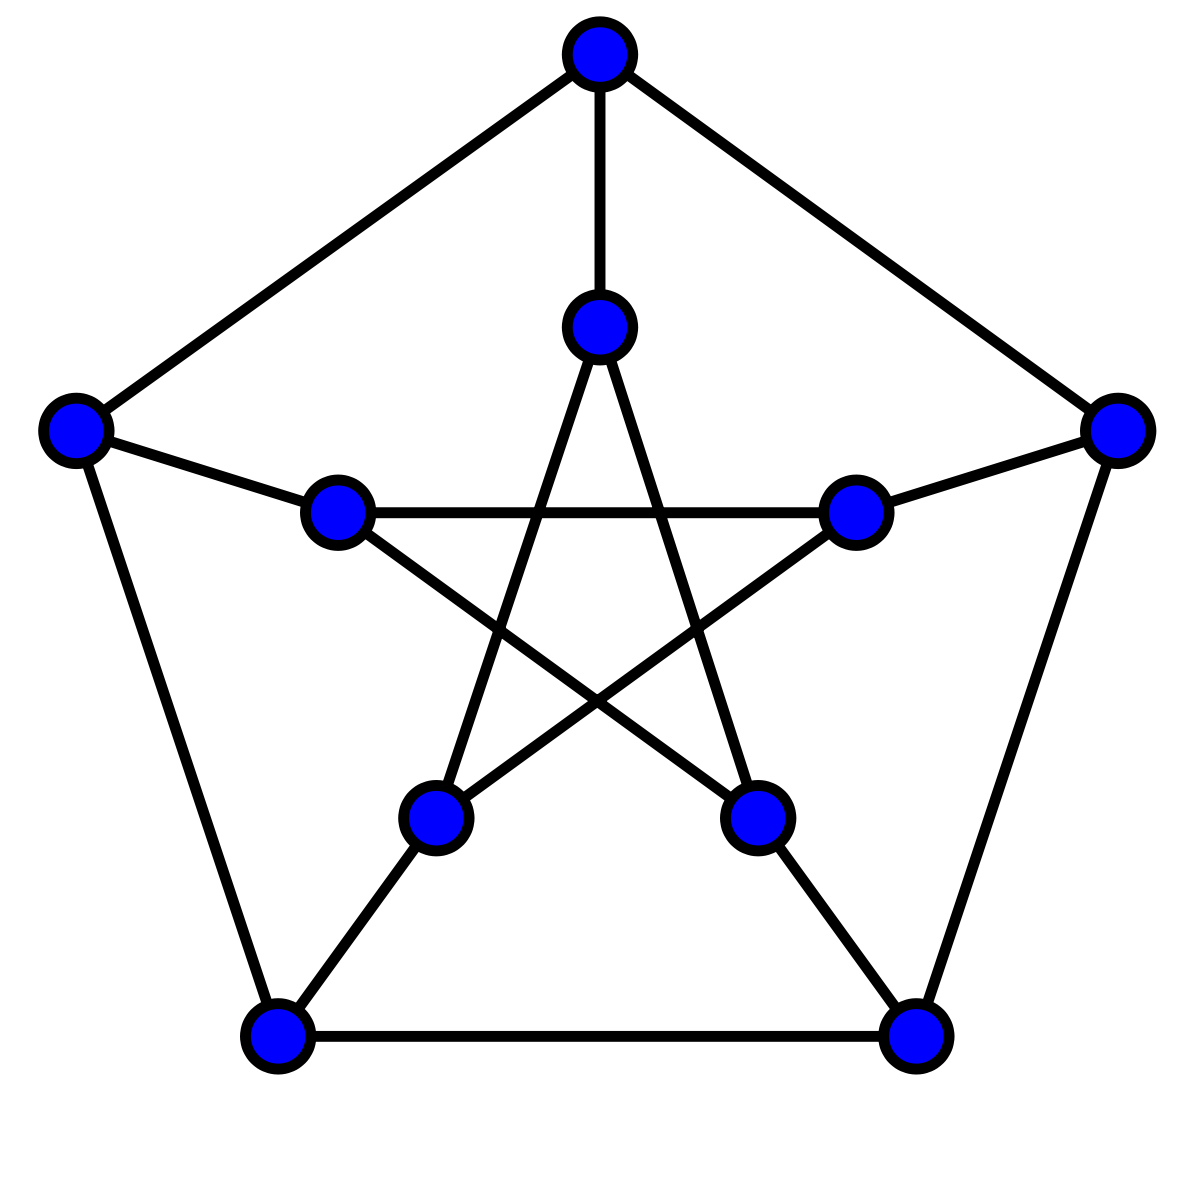
\includegraphics[width=1.2in]{petersen.png} \qquad \qquad (c) 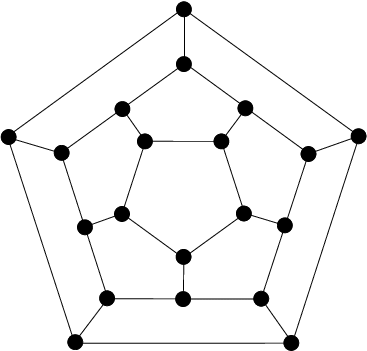
\includegraphics[width=1.2in]{dodecahedron.png}  \]

\end{enumerate}

\pagebreak


Recall that the \emph{degree} of a vertex $v$ of a graph $G=(V,E)$, denoted $\mathrm{deg}(v)$, is the number of edges containing $v$.
\begin{enumerate}

\setcounter{enumi}{2}

\item Give a simpler expression for $\sum_{v\in V}\mathrm{deg}(v)$.

\item You're at a party. Someone points out to you that the number of people at the party who have an odd amount of friends at the party is an even number. Explain to them why this always must be the case. (Assume friendship is symmetric, i.e., A is friends with B if and only if B is friends with A.)

\item Explain the relevance of the last problem to the question of when a graph has an Eulerian walk/circuit.

\end{enumerate}

\end{document}
